\documentclass[journal,11pt,twocolumn]{IEEEtran}

\usepackage{enumitem}
\usepackage{amsmath}
\usepackage{amssymb}
\usepackage{graphicx}
\providecommand{\pr}[1]{\ensuremath{\Pr\left(#1\right)}}
\providecommand{\cbrak}[1]{\ensuremath{\left\{#1\right\}}}
\providecommand{\brak}[1]{\ensuremath{\left(#1\right)}}
\providecommand{\cdf}[2]{\ensuremath{F_{#1}\left(#2\right)}}

\title{Assignment 6}
\author{Velma Dhatri Reddy \\ \normalsize AI21BTECH11030 \\ \vspace*{10pt} \Large CBSE Probability Grade 12}
\begin{document}
\maketitle
\textbf{Exercise 13.2.5:}
A die marked 1,2,3 in red and 4,5,6 in green is tossed. Let A be the event, ‘the number is even’, and B be the event, ‘the number is red’. Are A and B independent?

\textbf{Solution:} Let the random variable $X$ denote the number that appears on rolling the die. The sample space is $S = \cbrak{1, 2, 3, 4, 5, 6}$.
Hence, using pmf from Fig.\ref{fig:pmf}

Event A: The number is even
The sample space for event A is \cbrak{2,4,6}.
\begin{align}
    \pr{X \in A}&= \sum_{i = 1}^{i = 3}\pr{X = 2\times i}\\
    &= 3\times \dfrac{1}{6}\\
    &= \dfrac{3}{6}\\
    &= \dfrac{1}{2}
\end{align}

Event B: The number is red
The sample space for event B is \cbrak{1,2,3}.
\begin{align}
    \pr{X \in B}&= \sum_{i = 1}^{i = 3}\pr{X = i}\\
    &= 3\times \dfrac{1}{6}\\
    &= \dfrac{3}{6}\\
    &= \dfrac{1}{2}
\end{align}

Two events A and B are independent if 
$\pr{X \in AB } = \pr{X \in A}\times\pr{X \in B}$

\begin{align}
    AB = \cbrak{2}
\end{align}
    
\begin{align}
    \pr{X \in AB} &= \frac{n\brak{x \in AB}}{n\brak{x \in S}}\\
    &= \frac{1}{6}
\end{align}

\begin{multline}
    \pr{X \in A}\times\pr{X \in B} = \dfrac{1}{2}\times\dfrac{1}{2} = \dfrac{1}{4}\\
    \neq \pr{X \in AB } = \dfrac{1}{6}
\end{multline}
Hence, A and B are dependent events.

\begin{figure}[!ht]
\centering
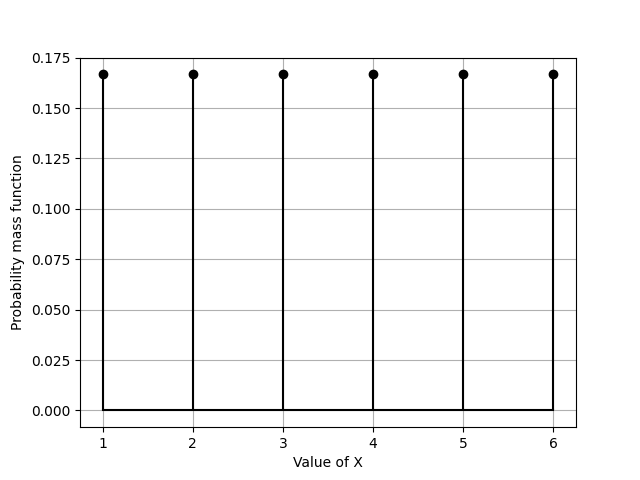
\includegraphics[width=\columnwidth]{figs/pmf.png}
\caption{Plot of the PMF of an unbiased die}
\label{fig:pmf}
\end{figure}
\end{document}